%%%%%%%%%%%%%%%%%%%%%%%%%%%%%%%%%%%%%%%%%
% Medium Length Professional CV
% LaTeX Template
% Version 2.0 (8/5/13)
%
% This template has been downloaded from:
% http://www.LaTeXTemplates.com
%
% Original author:
% Trey Hunner (http://www.treyhunner.com/)
%
% Important note:
% This template requires the resume.cls file to be in the same directory as the
% .tex file. The resume.cls file provides the resume style used for structuring the
% document.
%
%%%%%%%%%%%%%%%%%%%%%%%%%%%%%%%%%%%%%%%%%

%----------------------------------------------------------------------------------------
%	PACKAGES AND OTHER DOCUMENT CONFIGURATIONS
%----------------------------------------------------------------------------------------

\documentclass{resume} % Use the custom resume.cls style

\usepackage{graphicx}
\usepackage{float}
\usepackage{enumitem}
\usepackage{gensymb}
\usepackage{hyperref}
\hypersetup{
	colorlinks=true,    
	urlcolor=black,
}
\usepackage[left=0.4 in,top=0.4in,right=0.4 in,bottom=0.4in]{geometry} % Document margins
\newcommand{\tab}[1]{\hspace{.2667\textwidth}\rlap{#1}} 
\newcommand{\itab}[1]{\hspace{0em}\rlap{#1}}
\renewcommand{\baselinestretch}{1}
\name{\fangsong 黄屹 (E\lowercase{aston})} % Your name
%\address{123 Pleasant Lane \\ City, State 12345} % Your secondary addess (optional)
\address{\fangsong 个人网站:\url{www.eastonhy.com} \\ 电子邮箱:eastonhwang@gmail.com }
% In your preamble (before \begin{document})
\usepackage{amsmath}


\begin{document}

%\begin{minipage}{0.8\linewidth} %替换了原来的!htb
%	\centering
%  	\fontsize{20.0pt}\textbf{黄屹}\\
%  	+86 18041101930 \\ e1010591@u.nus.edu
%	%\caption{Illustration of nature ecological intelligent surveillance system} %actual scense rendering
%\end{minipage}
%\begin{minipage}{0.1\linewidth} %替换了原来的!htb
%	\centering
%	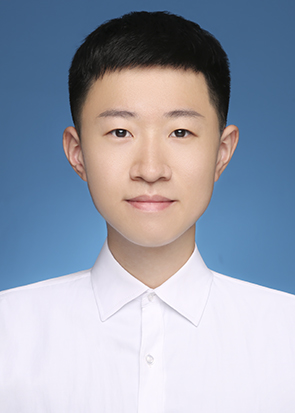
\includegraphics[width= 1in]{HY.jpg}
%	%\caption{Illustration of nature ecological intelligent surveillance system} %actual scense rendering
%\end{minipage}

%----------------------------------------------------------------------------------------
%	OBJECTIVE
%----------------------------------------------------------------------------------------
%\begin{figure}[b] %替换了原来的!htb
%	\centering
%	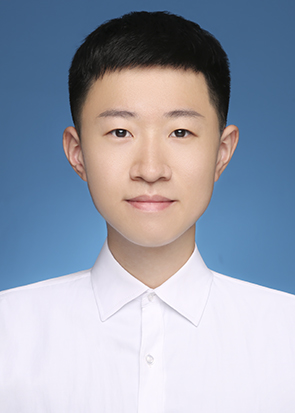
\includegraphics[width= 1in]{HY.jpg}
%	%\caption{Illustration of nature ecological intelligent surveillance system} %actual scense rendering
%	\label{women and sheep}
%\end{figure}

%----------------------------------------------------------------------------------------
%	EDUCATION SECTION
%----------------------------------------------------------------------------------------

\begin{rSection}{\fangsong 教育经历}

{\bf {\fangsong 研究生 - 机械工程}} \hfill {\em 2022. 8 - 2024. 1}\\ 
{\fangsong 新加坡国立大学 - 设计与工程学院}

{\bf {\fangsong 本科 - 机械设计制造及其自动化}} \\
{\fangsong 大连理工大学 - 机械工程学院} \hfill {\em {2018. 9 - 2021. 7}}\\
{\fangsong 新加坡国立大学苏州研究院}\hfill {\em 2021. 9 - 2022. 7}\\
\end{rSection}

\vspace{-1em}
%----------------------------------------------------------------------------------------
%	TECHNICAL STRENGTHS SECTION
%----------------------------------------------------------------------------------------

\begin{rSection}{\bf{\fangsong 技能}}
Unity3D, ANSYS (Workbench $\&$ APDL), Python, MATLAB, Arduino, Solidworks, CAD, Android Studio, HTML.  \\
\end{rSection}

\vspace{-1em}

%----------------------------------------------------------------------------------------
%	WORK EXPERIENCE SECTION
%----------------------------------------------------------------------------------------



\begin{rSection}{\bf {\fangsong 研究经历}}
\begin{rSubsection}{\bf {\fangsong 数字孪生与有限元分析结合}}{\fangsong 新加坡国立大学, 新加坡}
{\bf {\fangsong 研究生项目, 指导老师: Prof. Andrew Y.C. Nee \& Prof. Ong Sok Khim}  }{2022 - 2023}
	\item{\fangsong 关键词:数字孪生,结构健康监测,有限元分析,机器学习,代理模型。}\\
\end{rSubsection}

\begin{rSubsection}{\bf {\fangsong 基于机器视觉的表面质量检测}}{{\fangsong 新国大苏研院, 苏州}}
{\bf {\fangsong 本科生毕业设计, 指导老师: Prof. Wen Feng Lu}  }{2021 - 2022}
	\item{\fangsong 关键词:数字孪生,结构健康监测,有限元分析,机器学习,代理模型。}\\
\end{rSubsection}

\begin{rSubsection}{\bf {\fangsong 设计一种高度可调节的小凳}}{\fangsong 大连理工大学, 大连}
{\bf \fangsong 大学生创新创业项目,指导老师: 祝铁丽博士}{2021 - 2022}
	\item{\fangsong 关键词:结构设计与优化。}\\
\end{rSubsection}

\begin{rSubsection}{\bf \fangsong 基于多传感器数据的材料损伤建模}{\fangsong 大连理工大学, 大连}
{\bf \fangsong 国家级大学生创新创业项目,指导老师: 刘巍教授}{2020 - 2021}
	\item{\fangsong 关键词:CFRP的钻孔,多传感器测量,机器学习。}\\
\end{rSubsection}

\end{rSection}

\begin{rSection}{\fangsong 课程项目}
	
	\begin{rSubsection}{}{}
		{}{}
		\item {\fangsong {\bf 基于数据驱动机器学习的时空预测}\\ 课程名称: Data-Driven Engineering and Machine Learning}\\
		
		\item {\fangsong {\bf 基于声学分析的增材制造参数预测}\\ 课程名称: Engineering Acoustics}\\
		
		\item {\fangsong {\bf 产品碳排放分析和优化}\\ 课程名称: Sustainable Product Design $\&$ Manufacturing}\\
		
		\item {\fangsong {\bf 四足机器人的结构设计与分析} \\ 课程名称: 机械设计1课程设计}\\
		
		\item {\fangsong {\bf 加速器的设计与优化}\\ 课程名称: 机械设计2课程设计}\\
	\end{rSubsection}
	
	%\newpage
	
\end{rSection}

%----------------------------------------------------------------------------------------

\begin{rSection}{\fangsong 其他经历}
	
	\begin{rSubsection}{}{}
		{}{}
		\item {\fangsong {\bf 中国机器人及人工智能大赛}\\ 智慧农业比赛(田间自动巡航),指导老师:王龙飞博士\&刘胜蓝教授}\\
		
		\item {\fangsong {\bf Kaggle竞赛}\\UW-Madison GI Tract Image Segmentation (UWMGI)}\\
		
		\item {\fangsong {\bf 大连理工大学校级自强社}\\副社长 (大三), 事务部副部长 (大二), 外联部干事 (大一)}\\
	\end{rSubsection}
	
\end{rSection}
%----------------------------------------------------------------------------------------
\newpage
\begin{rSection}{\fangsong 荣誉}

\begin{rSubsection}{}{}
{}{}
  \item {\fangsong 中国机器人及人工智能大赛一等奖}\\
  \item {\fangsong 大连理工大学成绩优秀二等奖学金}\\
  \item {\fangsong Kaggle竞赛UWMGI项目铜牌(前6\%)}\\
  \item {\fangsong 大连理工大学校级自强社“优秀社干”荣誉称号}\\
\end{rSubsection}
\end{rSection}

%----------------------------------------------------------------------------------------
\begin{rSection}{\fangsong 成果}
\begin{rSubsection}{}{}
{}{}
	\item {{\bf Y. Huang}, 'Intelligent Machine Vision for Detection of Steel Surface Defects with Deep Learning,' 2023 IEEE International Conference on Smart Internet of Things (SmartIoT), Xining, China, 2023, pp. 326-327, doi: 10.1109/SmartIoT58732.2023.00059.}\\
  \item {\fangsong 祝铁丽,黄屹,闫开,孙先成.便携折叠床椅的研制[J].科学与技术,2022(30).}\\
  \item {\fangsong 祝铁丽,司海仑,黄屹,孙先成.高度可调节小凳的研制[J].科学与生活,2021(25).}\\
  \item {\fangsong 祝铁丽,时灏烨,林宏彬,李传杰,黄屹,孙先成. 握笔姿势矫正器[P]. 辽宁省:CN214449773U,2021-10-22.}\\
\end{rSubsection}
\end{rSection}

%----------------------------------------------------------------------------------------

\end{document}

